\mysection{課題1}
\begin{enumerate}
  \item 計算開始後500ステップまで50ステップ毎の温度分布、速度ベクトルの様子を図示せよ。\\
  50ステップ毎の温度分布、速度ベクトルの様子を図\ref{im1}に示す。\\青色が低温側で赤色が高温側である。
  \begin{figure}[htb]
    \begin{center}
    \subfigure[ステップ数$=50$の時]{
    \includegraphics[width=.2\columnwidth]{img/1/50.png}
    }
    \subfigure[ステップ数$=100$の時]{
    \includegraphics[width=.2\columnwidth]{img/1/100.png}
    }
    \subfigure[ステップ数$=150$の時]{
    \includegraphics[width=.2\columnwidth]{img/1/150.png}
    }
    \subfigure[ステップ数$=200$の時]{
    \includegraphics[width=.2\columnwidth]{img/1/200.png}
    }
    \subfigure[ステップ数$=250$の時]{
    \includegraphics[width=.2\columnwidth]{img/1/250.png}
    }
    \subfigure[ステップ数$=300$の時]{
    \includegraphics[width=.2\columnwidth]{img/1/300.png}
    }
    \subfigure[ステップ数$=350$の時]{
    \includegraphics[width=.2\columnwidth]{img/1/350.png}
    }
    \subfigure[ステップ数$=400$の時]{
    \includegraphics[width=.2\columnwidth]{img/1/400.png}
    }
    \subfigure[ステップ数$=450$の時]{
    \includegraphics[width=.2\columnwidth]{img/1/450.png}
    }
    \subfigure[ステップ数$=500$の時]{
    \includegraphics[width=.2\columnwidth]{img/1/500.png}
    }
    \caption{50ステップ毎の温度分布・速度ベクトルの様子}
    \label{im1}
    \end{center}
  \end{figure}
  図\ref{im1}より、ステップ数が増加すると高温の空気と低温の空気の混合が進展することが分かる。ステップ数が350程度になると、温度分布が一定になる。
  速度ベクトルの大きさは、ステップ数が増加するごとに大きくなり、温度分布が一定になると減少傾向になる。
  \item $Gr$ を変化させ、定常状態における高温壁と低温壁の平均$Nu$数と$Gr$数の関係を図に示せ。\\$(10^3 < Ra < 10^5)$\\
  はじめに、$Gr$数を変化させた時の高温壁と低温壁の平均$Nu$数と$Gr$数の関係を表\ref{tab1}に示す。
  \newpage
  \begin{table}[h]
    \centering
    \caption{$Gr$数を変化させた時の高温壁と低温壁の平均$Nu$数と$Gu$数の関係}
    \begin{tabular}[t]{lrr}
    \toprule
    $Re$数&$Gr$数&平均$Nu$数\\
    \midrule
    $1.0 \times 10^3$&1428.57&4.44229\\
    $2.5 \times 10^3$&3571.43&5.49029\\
    $5.0 \times 10^3$&7142.86&6.81448\\
    $7.5 \times 10^3$&10714.3&7.75238\\
    $1.0 \times 10^4$&14285.7&8.47924\\
    $2.5 \times 10^4$&35714.3&11.1318\\
    $5.0 \times 10^4$&71428.6&13.5280\\
    $7.5 \times 10^4$&107143&15.0941\\
    $1.0 \times 10^5$&142857&16.2690\\
    \bottomrule
    \end{tabular}
    \label{tab1}
  \end{table}
  次に、平均$Nu$数と$Gr$数の関係を図\ref{graph1}に示す。
  \begin{figure}[htbp]
    \begin{center}
    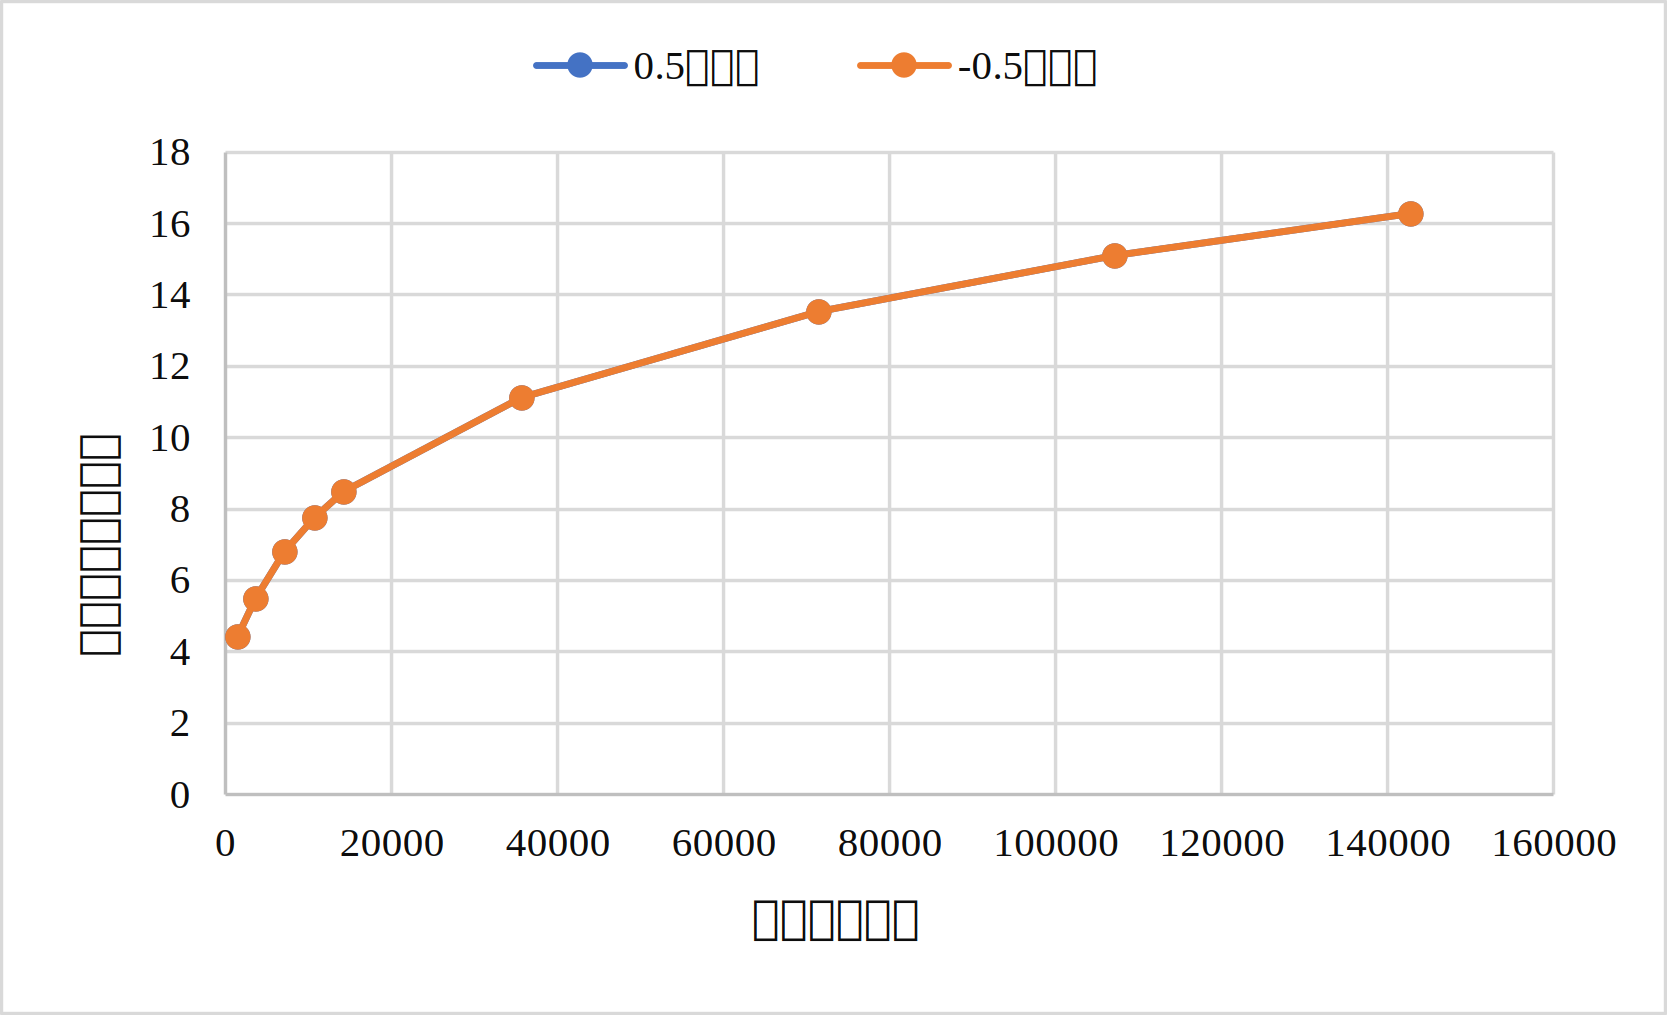
\includegraphics[width=0.85\linewidth]{img/2/1_2.png}
    \caption{平均$Nu$数と$Gr$数の関係}
    \label{graph1}
    \end{center}
  \end{figure}
  \\図\ref{graph1}より、グラスホフ数の増加に対して、平均ヌッセルト数は単調増加傾向にある。
  \item メッシュサイズを変化させ、$Ra = 10^5$ において$Nu$数が変化する様子を調べよ。\\(最初は20になっている。5 → 100)\\
  $Ra=10^5$において$Nu$数が変化する様子を図\ref{im2}に示す。\\
  メッシュ数が0~40の値域の時、平均ヌッセルト数は単調増加傾向である。
  しかし、メッシュ数の地域が50以上になると、平均ヌッセルト数の値の変化傾向が定まらず、振動する。
  これは、ヌッセルト数の導出式において、メッシュ数を無限大とした時の極限値が収束も発散もしないためだと考えられる。
  \newpage
  \begin{figure}[htb]
    \begin{center}
    \subfigure[メッシュサイズを0~50まで変化させた時の平均$Nu$数の変化]{
    \includegraphics[width=.85\columnwidth]{img/3/1_3_1.png}
    }
    \subfigure[メッシュサイズを50~100まで変化させた時の平均$Nu$数の変化]{
    \includegraphics[width=.85\columnwidth]{img/3/1_3_2.png}
    }
    \caption{$Ra=10^5$において$Nu$数が変化する様子}
    \label{im2}
    \end{center}
  \end{figure}
  \item 図\ref{1_4_instruction}のモデルに関して計算を行い、定常状態の温度分布と速度ベクトルの様子を示せ。\\(メッシュ $40 \times 40$、$Re = 500$)\\
  定常状態の温度分布と速度ベクトルの様子を図\ref{img3}に示す。
  左上部分から、冷気が流入し、内面の常温空気と混合する過程で渦が発生している。実行サイクル数を大きくすることで、内面全体に渦が広がり、右下部から流出すると考えられる。
  
  \newpage
  \begin{figure}[htbp]
    \begin{center}
    \includegraphics[width=0.5\linewidth]{img/4/1_4_instruction.png}
    \caption{モデル}
    \label{1_4_instruction}
    \end{center}
  \end{figure}
  \begin{figure}[htbp]
    \begin{center}
    \includegraphics[width=0.4\linewidth]{img/4/1_4_3_kai.png}
    \caption{モデルの定常状態の温度分布と速度ベクトルの様子}
    \label{img3}
    \end{center}
  \end{figure}

  \item 演習2の課題について説明せよ。\\
  サウナ室内の熱気の流れについて解析する。
  具体的には、1 熱石を置いてどれぐらいの時間で室内が温まるか、2 サウナ室に窓を付けるとどうなるのか(何処なら付けてよくて良くないか)3 熱石を置く場所を変えるとどうなるのかを検証する。
  サウナ室を模した2次元平面上に熱源(熱石)を置き、窓に関しては、強制的に速度を付けるのではなく、格子間の速度が一定である自由流出の条件で設定する。\\
  これらをサンプルプログラムのパラメータに定義し、実行サイクルごとに温度分布・速度ベクトルの様子を観察することで明らかにする。
\end{enumerate}